\subsection{Proposed Pilgrim Oil Pipelines}\label{subec:pilgrim}
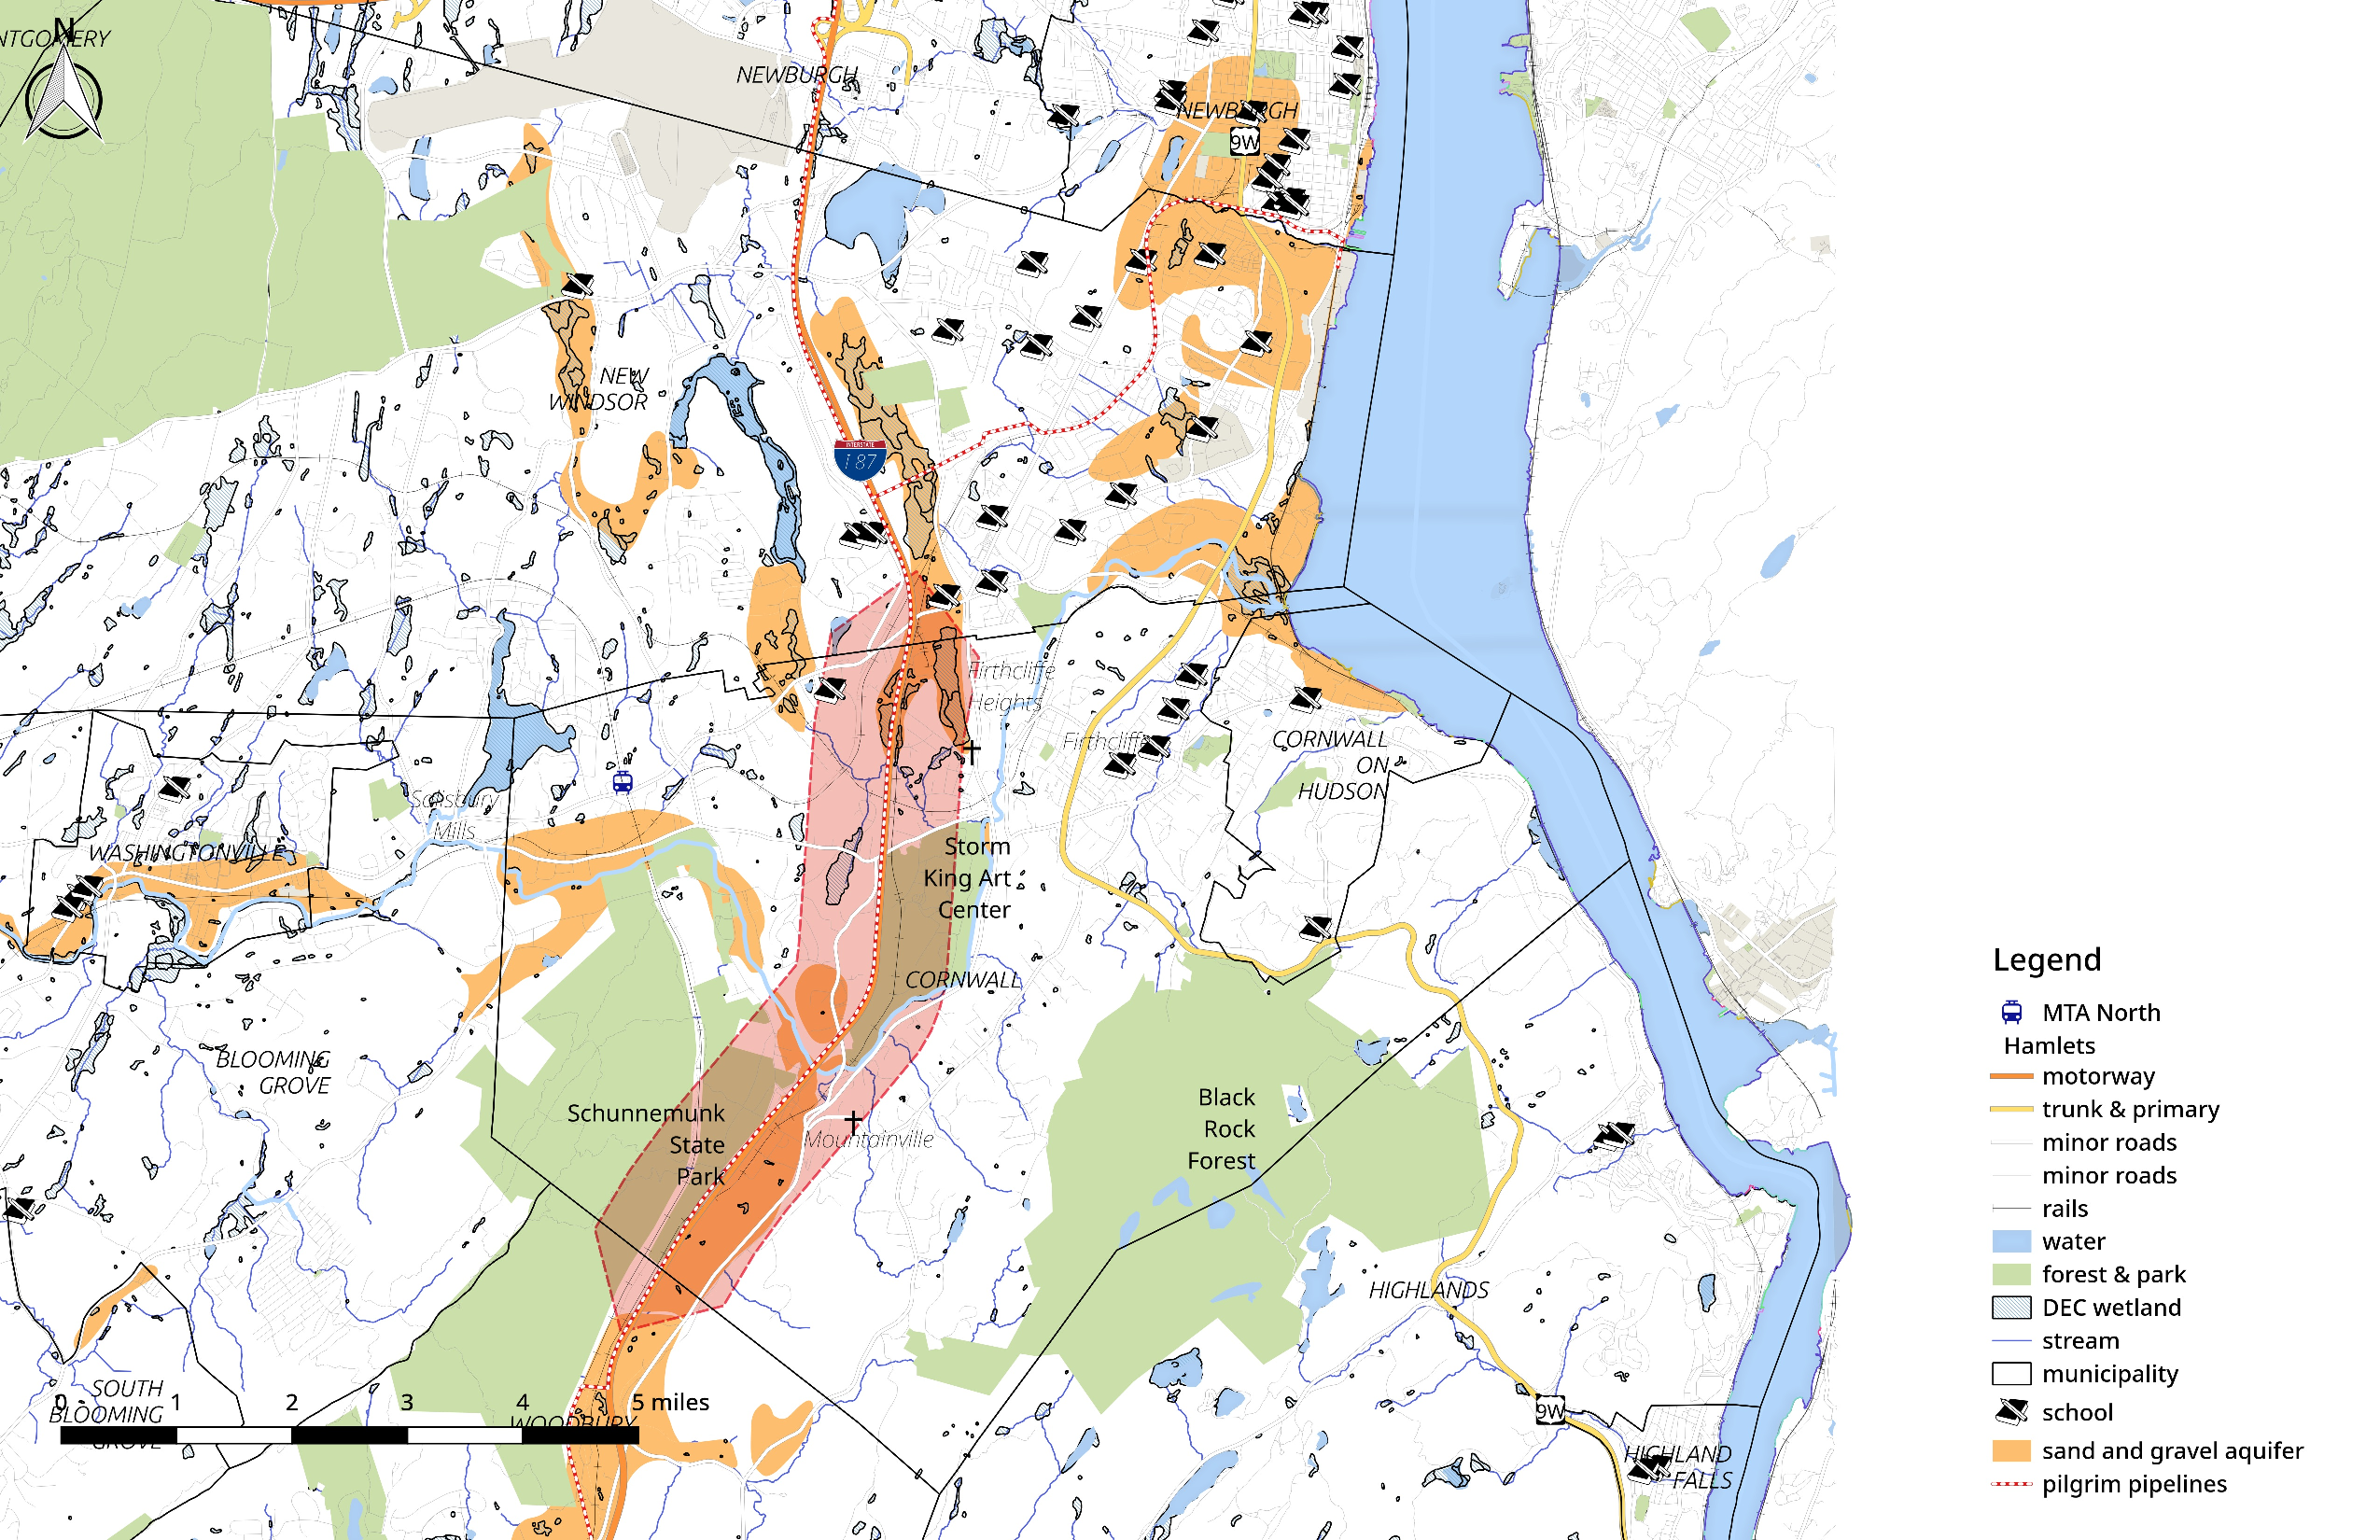
\includepdf[pages=-,fitpaper]{cornwall_maps/proposed_pilgrim_oil_pipelines.pdf}
\label{map:proposedoilpipelines}
This map shows planned fossil fuel infrastructure and its proximity to sand and 
gravel aquifers, public institutions and other important natural areas. The 
proposed Pilgrim Oil Pipelines would carry both refined petroleum products 
(gasoline, diesel, heating oil, and kerosene) and crude oil underground between 
Linden, NJ and Albany, NY along the NYS Thruway. The project’s co-lead 
agencies, \gls{nysta} and \gls{nysdec} determined the project would have 
``potentially significant impact on the environment'' and hence issued a 
``Positive Declaration`` under Article 8 of the Environmental Conservation 
Law. A ''Positive Declaration`` requires a full Environmental Impact Statement 
(EIS) with a public scoping requirement and public comment period. The pipelines 
would be 356 miles long, with 116.4 miles being in New York State, with 5 
laterals, 4 pump stations, 10 meter stations and 35 permanent access roads. 
During construction there would be 50 temporary access roads and 7 major 
construction zones/staging areas. Each pipeline would be 20 inches in diameter 
and have the potential to transport 8.4 million gallons per day (200,000 
barrels/day). The pipelines would cross 257 waterways and would be run very 
close to water supplies of municipalities. There are also 296 (9.2 linear miles)
crossings of wetlands; including 25 crossings of \gls{nysdec}protected 
freshwater wetlands (approximately 19 along mainline pipelines and 6 along 
laterals). If pipelines were constructed more solidly or their leak detection 
systems were better then this might not be an issue. Recent data suggests that 
pipelines are prone to leaking and sometimes days go by before a leak is 
detected and is responded to.

From the south, the pipelines would run adjacent to Schunemunk State Park and 
Storm King Arts Center which are important recreation sites and home to flora 
and fauna. A little less than 5 miles (4.6) of the pipeline would bisect the 
Town’s boundary. Much of the pipelines in Cornwall would be located on top of 
sand and gravel aquifers. The pipeline also traverses across 4 waterways in 
Cornwall and 5 points that are designated as high yielding well sites would be 
within one mile of the proposed pipelines. Two churches and the Cornwall High 
School are within a 0.5 mile risk zone as can be seen on the map. The half mile 
risk zone was added to the map to give viewers an idea off how close they would 
be to the dangers of a leak or an explosion.

In the Town of New Windsor, the lateral would run adjacent to the Quassaick 
Creek which is an important habitat for eel species. Much of the pipelines’ path 
would be built on top of a sand and gravel aquifer which is described as 
“Stratified clay and silt with no or thin layers of sand and gravel at land 
surface and below the water table”. A spill on top of a sand and gravel aquifer 
would risk serious contamination of the groundwater.

\subsection{Proposed Anchorage Sites on the Hudson 
River}\label{subsec:anchorages}
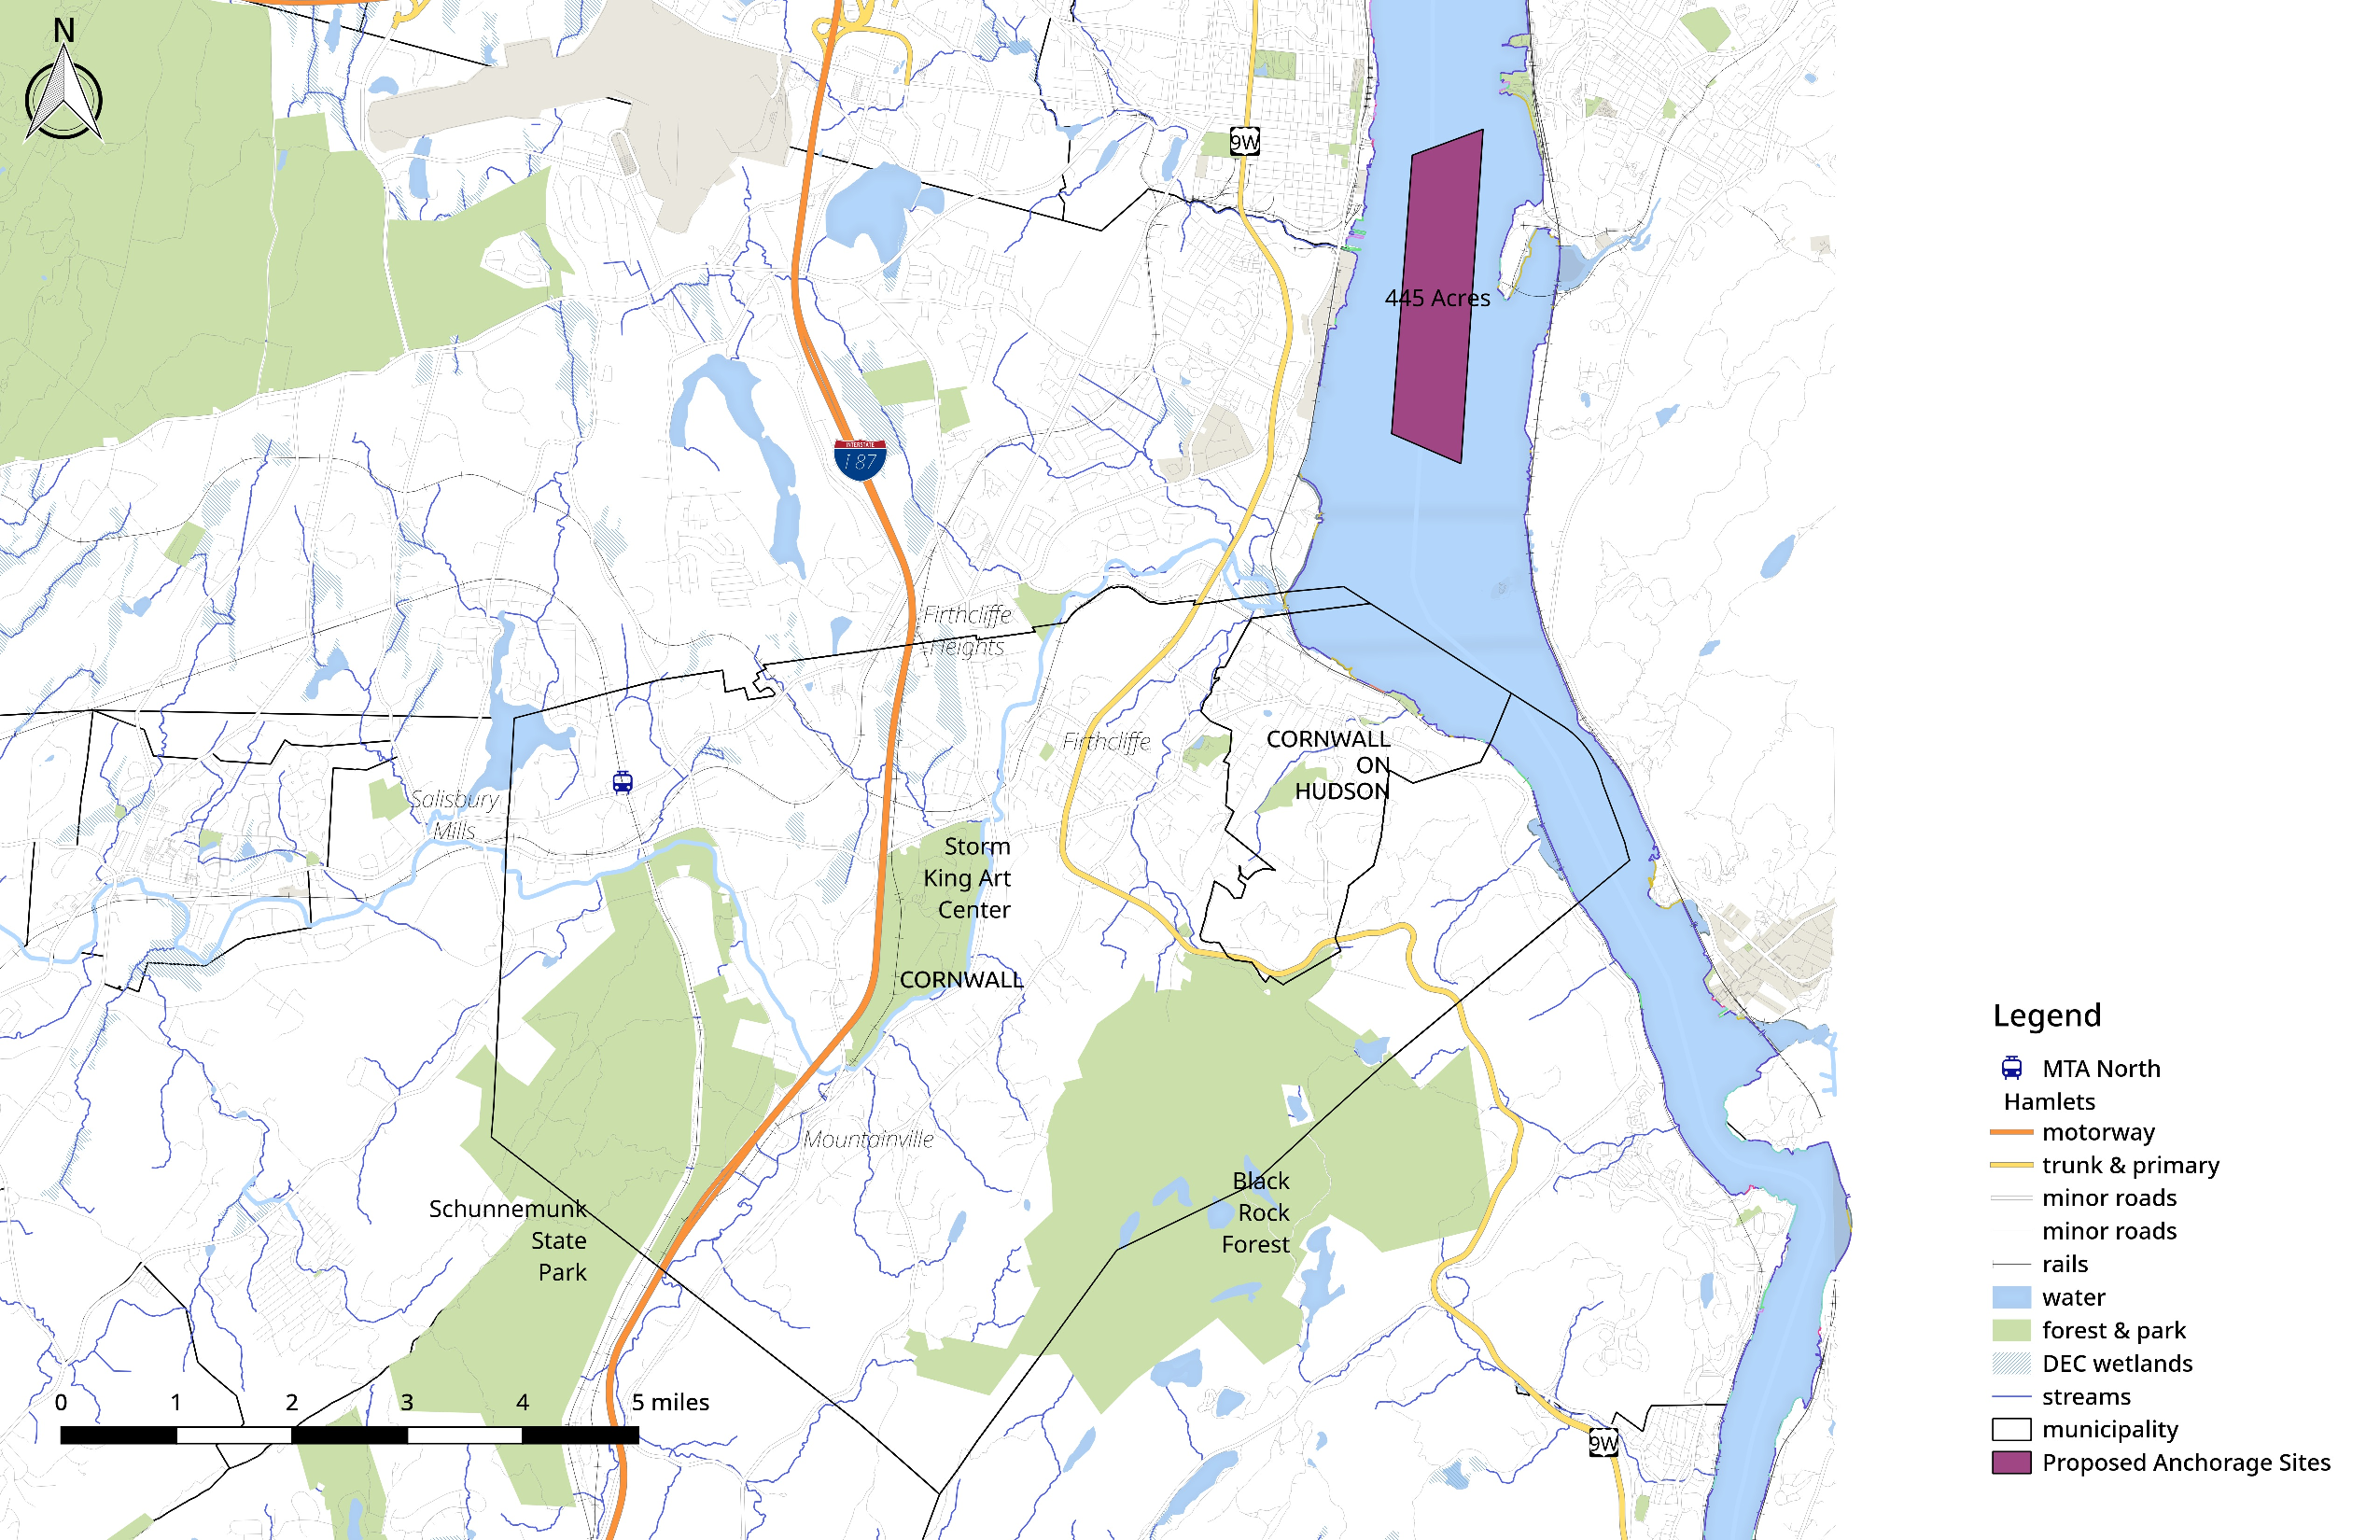
\includepdf[pages=-,fitpaper]{cornwall_maps/proposed_anchorages.pdf}\label{map:proposedanchorages}
This map displays two of the 42 long-term proposed anchorage sites on the Hudson 
River that was submitted by the The Maritime Association of the Port of New 
York/New Jersey to the US Coast Guard in January 2016. The lifting of the oil 
export ban has increased barge traffic on the Hudson River, increasing the risk 
of an accident. The Newburgh hub would have room for a total of 8 barges, with 
space for 5 barges being moored adjacent to the City of Newburgh and 3 moored 
north of the Newburgh/Beacon Bridge. The first area of anchorage sites would 
make 445.34 acres of the Hudson available to barges and the latter would make an 
additional 305 acres of the Hudson available. These barges most likely will 
transport oil and environmental groups have warned that besides the risk of 
spills and explosions that this will turn the Hudson River into a parking lot. 
Due to backlash from engaged citizens, the Coast Guard scrapped the proposal and 
convened a Ports and Waterway Safety Assessment (PAWSA). Multiple workshops were 
held to gain stakeholder insight and plan for a safe Hudson River. Furthermore, 
Governor Andrew Cuomo signed a bill in October, 2017 which gives the 
\gls{nysdec} authority to regulate oil barges on the Hudson River and instructs 
the agency to enact ''tanker avoid zones``.
